\chapter{分立半导体元件}

\section{Diode}

\subsection{Zener}

A Zener diode is a special type of diode designed to reliably allow current to flow "backwards" (inverted polarity) when a certain set reverse voltage, known as the Zener voltage, is reached. \footnote{本节内容源于 Wikipedia。}

Zener diodes are manufactured with a great variety of Zener voltages and some are even variable. Some Zener diodes have an abrupt, heavily doped p–n junction with a low Zener voltage, in which case the reverse conduction occurs due to electron quantum tunnelling in the short distance between p and n regions − this is known as the Zener effect, after Clarence Zener. Diodes with a higher Zener voltage have lighter doped junctions which causes their mode of operation to involve avalanche breakdown. Both breakdown types are present in Zener diodes with the Zener effect predominating at lower voltages and avalanche breakdown at higher voltages.

They are used to generate low-power stabilized supply rails from a higher voltage and to provide reference voltages for circuits, especially stabilized power supplies. They are also used to protect circuits from overvoltage, especially electrostatic discharge.

\BlockDesc{构造}

The Zener diode's operation depends on the heavy doping of its p–n junction. The depletion region formed in the diode is very thin (<1 µm) and the electric field is consequently very high (about 500 kV/m) even for a small reverse bias voltage of about 5 V, allowing electrons to tunnel from the valence band of the p-type material to the conduction band of the n-type material.

At the atomic scale, this tunneling corresponds to the transport of valence band electrons into the empty conduction band states; as a result of the reduced barrier between these bands and high electric fields that are induced due to the high levels of doping on both sides.[3] The breakdown voltage can be controlled quite accurately by the doping process. Adding impurities, or doping, changes the behaviour of the semiconductor material in the diode. In the case of Zener diodes, this heavy doping creates a situation where the diode can operate in the breakdown region. While tolerances within 0.07\% are available, commonly available tolerances are 5\% and 10\%. Breakdown voltage for commonly available Zener diodes can vary from 1.2 V to 200 V.

For diodes that are lightly doped, the breakdown is dominated by the avalanche effect rather than the Zener effect. Consequently, the breakdown voltage is higher (over 5.6 V) for these devices.

\BlockDesc{使用}

\begin{wrapfigure}{r}{2cm}
   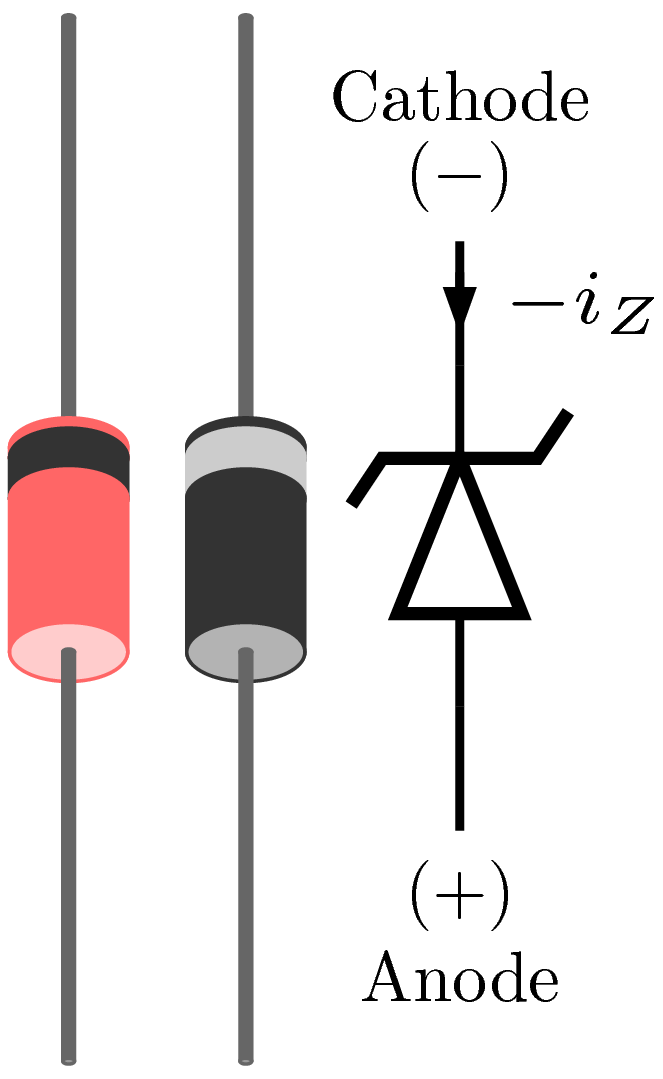
\includegraphics[width=1.5cm,height=3cm]{Zener_3D_and_ckt}
   % \caption{Zener 二极管器件及符号}
\end{wrapfigure}

Zener diodes are widely used as voltage references and as shunt regulators to regulate the voltage across small circuits. When connected in parallel with a variable voltage source so that it is reverse biased, a Zener diode conducts when the voltage reaches the diode's reverse breakdown voltage. From that point on, the low impedance of the diode keeps the voltage across the diode at that value.

\Figure[caption={Zener 稳压电路}, label={fig:zener-stabilized-circuit}, width=0.4]{Zener_diode_voltage_regulator}

In this circuit, a typical voltage reference or regulator, an input voltage, Uin (with + on the top), is regulated down to a stable output voltage Uout. The breakdown voltage of diode D is stable over a wide current range and holds Uout approximately constant even though the input voltage may fluctuate over a wide range. Because of the low impedance of the diode when operated like this, resistor R is used to limit current through the circuit.

In the case of this simple reference, the current flowing in the diode is determined using Ohm's law and the known voltage drop across the resistor R;

\[
I_{diode} = \frac{U_{in} - U_{out}}{R}
\]

The value of R must satisfy two conditions:

\begin{enumerate}
\item R must be small enough that the current through D keeps D in reverse breakdown. The value of this current is given in the data sheet for D. For example, the common BZX79C5V6 device, a 5.6 V 0.5 W Zener diode, has a recommended reverse current of 5 mA. If insufficient current exists through D, then Uout is unregulated and less than the nominal breakdown voltage (this differs from voltage-regulator tubes where the output voltage is higher than nominal and could rise as high as Uin). When calculating R, allowance must be made for any current through the external load, not shown in this diagram, connected across Uout.
\item R must be large enough that the current through D does not destroy the device. If the current through D is ID, its breakdown voltage VB and its maximum power dissipation Pmax correlate as such: $I_{D}V_{B}<P_{max}$.
\end{enumerate}

A load may be placed across the diode in this reference circuit, and as long as the Zener stays in reverse breakdown, the diode provides a stable voltage source to the load. Zener diodes in this configuration are often used as stable references for more advanced voltage regulator circuits.

Shunt regulators are simple, but the requirements that the ballast resistor be small enough to avoid excessive voltage drop during worst-case operation (low input voltage concurrent with high load current) tends to leave a lot of current flowing in the diode much of the time, making for a fairly wasteful regulator with high quiescent power dissipation, suitable only for smaller loads.

These devices are also encountered, typically in series with a base-emitter junction, in transistor stages where selective choice of a device centered on the avalanche or Zener point can be used to introduce compensating temperature co-efficient balancing of the transistor p–n junction. An example of this kind of use would be a DC error amplifier used in a regulated power supply circuit feedback loop system.

Zener diodes are also used in surge protectors to limit transient voltage spikes.

\section{BJT}

\subsection{三极管分析步骤}

\subsubsection{静态工作点 DC 分析}

\subsubsection{动态小信号模型 AC 分析}

\subsection{共射}

\subsection{共集}

\subsection{共基}

\section{JFET}

\section{MOSFET}

